%%%%%%%%%%%%%%%%%%%%%%%%%%%%%%%%%%%%%%%%%
%
% CMPT xxx
% Some Semester
% Lab/Assignment/Project X
%
%%%%%%%%%%%%%%%%%%%%%%%%%%%%%%%%%%%%%%%%%

%%%%%%%%%%%%%%%%%%%%%%%%%%%%%%%%%%%%%%%%%
% Short Sectioned Assignment
% LaTeX Template
% Version 1.0 (5/5/12)
%
% This template has been downloaded from: http://www.LaTeXTemplates.com
% Original author: % Frits Wenneker (http://www.howtotex.com)
% License: CC BY-NC-SA 3.0 (http://creativecommons.org/licenses/by-nc-sa/3.0/)
% Modified by Alan G. Labouseur  - alan@labouseur.com
% Further modified by Brian Gormanly - brian.gormanly@marist.edu (2023.1)
%
%%%%%%%%%%%%%%%%%%%%%%%%%%%%%%%%%%%%%%%%%

%----------------------------------------------------------------------------------------
%	PACKAGES AND OTHER DOCUMENT CONFIGURATIONS
%----------------------------------------------------------------------------------------

\documentclass[10pt]{article} 

\usepackage[T1]{fontenc} % Use 8-bit encoding that has 256 glyphs
\usepackage[english]{babel} % English language/hyphenation
\usepackage{amsmath,amsfonts,amsthm,xfrac} % Math packages
%\usepackage{sectsty} % Allows customizing section commands
\usepackage{graphicx}
\usepackage[linesnumbered,commentsnumbered]{algorithm2e}
\usepackage{listings}
\usepackage{parskip}
\usepackage{lastpage}
%\allsectionsfont{\normalfont\scshape} % Make all section titles in default font and small caps.
\usepackage{titlesec}
\usepackage[margin=1.25in]{geometry}

\usepackage{fancyhdr} % Custom headers and footers
%\pagestyle{fancyplain} % Makes all pages in the document conform to the custom headers and footers

\fancyhead{} % No page header - if you want one, create it in the same way as the footers below
\fancyfoot[L]{} % Empty left footer
\fancyfoot[C]{} % Empty center footer
\fancyfoot[R]{page \thepage\ of \pageref{LastPage}} % Page numbering for right footer

\renewcommand{\headrulewidth}{0pt} % Remove header underlines
\renewcommand{\footrulewidth}{0pt} % Remove footer underlines
\setlength{\headheight}{13.6pt} % Customize the height of the header

%\numberwithin{equation}{section} % Number equations within sections (i.e. 1.1, 1.2, 2.1, 2.2 instead of 1, 2, 3, 4)
%\numberwithin{figure}{section} % Number figures within sections (i.e. 1.1, 1.2, 2.1, 2.2 instead of 1, 2, 3, 4)
%\numberwithin{table}{section} % Number tables within sections (i.e. 1.1, 1.2, 2.1, 2.2 instead of 1, 2, 3, 4)

\setlength\parindent{0pt} % Removes all indentation from paragraphs.

\binoppenalty=3000
\relpenalty=3000

%----------------------------------------------------------------------------------------
%	TITLE SECTION
%----------------------------------------------------------------------------------------

\newcommand{\horrule}[1]{\rule{\linewidth}{#1}} % Create horizontal rule command with 1 argument of height

\title{	
   \normalfont \normalsize 
   \textsc{CMPT 435 - Spring 2023 - Prof. Gormanly} \\[10pt] % Header stuff.
   \horrule{0.5pt} \\[0.25cm] 	% Top horizontal rule
   \huge Assignment One  \\     	    % Assignment title
   \horrule{0.5pt} \\[0.25cm] 	% Bottom horizontal rule
}

\author{Your Name \\ \normalsize Your.Name@Marist.edu}

\date{\normalsize\today} 	% Today's date.

\titleformat{\section}
  {\normalfont\fontsize{15}{15}\bfseries}{\thesection}{1em}{}
\titleformat{\subsection}
  {\normalfont\fontsize{12}{12}\bfseries}{\thesubsection}{1em}{}
\titleformat{\subsubsection}
  {\normalfont\fontsize{11}{11}\bfseries}{\thesubsubsection}{1em}{}

\begin{document}
\maketitle % Print the title

%----------------------------------------------------------------------------------------
%   start PROBLEM ONE
%----------------------------------------------------------------------------------------
\section{Problem One}

\subsection{The Data Structure}
An $n$-element array of integer pairs: ($currentCount$, $predecessorSum$) will, once initialized in the preprocessing step,  support \textsc{Member}, \textsc{Less}, and \textsc{Range} operations as described in Section \ref{operations} in $O(1)$ (constant) time.

For illustration, consider the case where $S = (1, 2, 3, 4, 7, 7, 7, 7, 7, 8, 9, 10, 10,10,10,10,10, 14, 16)$. \\
Here we have $m = 19$ elements in $S$ ranging in value from 1 through $n = 16$.
The array for $S$ after preprocessing is given in Figure~\ref{figure:array}.

% This is how we include a figure when 
% the file is in the same directory as this document (see array.png in file panel).
\begin{figure}[ht] 
   \centering 
   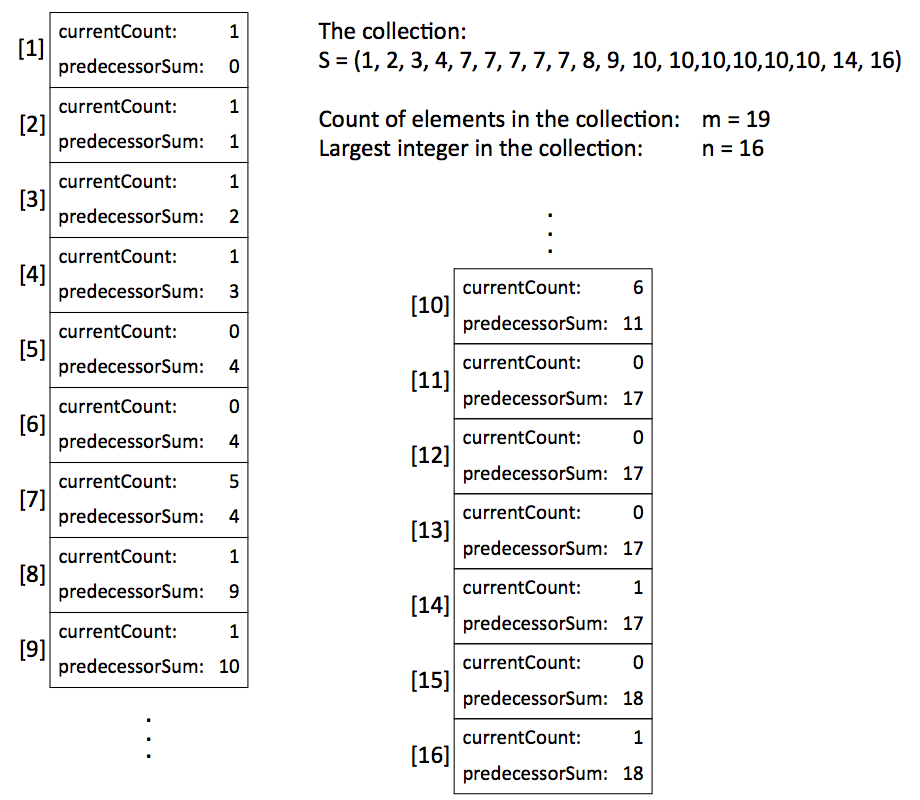
\includegraphics[width=11cm]{array}
   \caption{Example array built from 19 values, 10 of them unique.}
   \label{figure:array}
\end{figure}

\subsection{Preprocessing}
There are two preprocessing steps, \textsc{Tally} and \textsc{Predecessor Sum}, each of which is $O(m+n)$ as we will see in Equations \ref{equation:pass1} and \ref{equation:pass2} below.
This makes the overall performance $O(m+n)$ because 
$2 \cdot O(m+n) =\footnote{This is an abuse of the notation, but if it's okay in the CLRS~\cite{clrs} book I hope it's okay here.} O(m+n)$.

% Note bot the footnote and the citation in the above two lines.

\subsubsection{Pass one: Tally}
For each element $i$ in $S$ we'll store its number of occurrences at $A[i].currentCount$.

% This is an example of including an algorithm in your document.
\begin{algorithm}[H]
    \SetAlgoLined
    \caption{Tally}
    \label{algorithm:tally}
    \KwData{collection $S$}
    \KwResult{array $A$ containing tallys for each element $i$ in $S$ }
   
    allocate $A[n]$\;
    \For{$j \leftarrow 1$ \KwTo $n$}{
         $A[j].currentCount \leftarrow 0$\;
    }   
    \ForEach(// There are $m$ elements in $s$.){element i in S}{
         $A[i].currentCount \leftarrow A[i].currentCount + 1$\;
    }
\end{algorithm}

\textbf{Asymptotic Analysis} \\
We are given $m$ integer values (the size of the collection), each in the range $[1..n]$ (the size of the domain) and want to iterate over them, computing the tally for each.
Consider Algorithm~\ref{algorithm:tally}.
Line 1 executes in constant time.
Lines 2 through 4 execute in $O(n)$ time because we are iterating from 1 to $n$.  
Lines 5 through 7 execute in $O(m)$ time because we are iterating over all the elements of $S$, of which there are $m$.  

% This is how you include an equation:

So, for pass one, we have :
\begin{equation}   
   \label{equation:pass1}   
   \begin{split}
   O(pass1) & = constant + O(n) + O(m)\\
            & = O(n) + O(m)\\
            & = O(m+n)   
   \end{split}
\end{equation}

\subsubsection{Pass two: Predecessor Sum}
Once the tally is done we need to make another pass over $A$ to compute, for each $A[i] : i>1$, 
the sum of all of its predecessors ($A[1] .. A[i-1]$) and store that in $A[i].predecessorSum$.

\begin{algorithm}[H]
    \SetAlgoLined
    \caption{Predecessor Sum}
    \label{algorithm:predecessorSum}
    \KwData{array $A$ containing tallys for each element $i$ in $S$}
    \KwResult{a new and improved array $A$, now with the predecessor sums}
   
    $A[1].predecessorSum \leftarrow 0$\;
   \If {n > 1} {
       \For{$k\leftarrow 2$ \KwTo $n$}{
            $A[k].predecessorSum \leftarrow A[k-1].predecessorSum + A[k-1].currentCount$\;
        }   
   }
\end{algorithm}

\textbf{Asymptotic Analysis}\\
Looking at Algorithm~\ref{algorithm:predecessorSum}, line 1 is assignment, a constant time operation.
If lines 3 through 5 execute at all, they do so in $O(n)$ time because we make $n - 1$ iterations over line 4, which is assignment and array lookups, both constant time operations.
For pass two, we have :
\begin{equation}
   \label{equation:pass2}   
   \begin{split}       
       O(pass2) & = constant + O(n) \\
                & = O(n) \\
                & = O(m+n) \, \text{which is ok so long as $m > 0$}   
    \end{split}
\end{equation}


\subsection{Operations}\label{operations}

\subsubsection{Member}

\begin{algorithm}[H]
    \SetAlgoLined
    \caption{Member}
    \label{algorithm:member}
    \KwIn{parameter $i$}
    \KwData{a new and improved array $A$, replete with tallys and predecessor sums}
    \KwOut{$True$ if $i$ exists in $S$, $False$ otherwise}
     
    \eIf {$(i \ge 1) \land (i \le n)$} {
        return $(A[i].currentCount > 0)$\;
    } {
        return $False$\;
   }
\end{algorithm}

\textbf{Asymptotic Analysis}\\
Looking at Algorithm~\ref{algorithm:member}, line 1 consists of comparisons, which are constant time operations.
Line 2 is an array lookup and a comparison, both constant time operations.
The remaining parts of the algorithm (including the rest of line 2) are for program control, and not considered in this analysis. Since all parts of the algorithm execute in constant time, the whole thing executes in constant time and is therefore $O(1)$.

\subsubsection{Less}

\begin{algorithm}[H]
    \SetAlgoLined
    \caption{Less}
    \label{algorithm:less}
    \KwIn{parameter $i$}
    \KwData{a new and improved array $A$, replete with tallys and predecessor sums}
    \KwOut{The number of elements in $S$ that are strictly less than $i$.}
     
    \eIf {$(i \ge 1) \land (i \le n)$} {
        return $A[i].predecessorSum$\;
    } {
        return 0\;
   }
\end{algorithm}

\textbf{Asymptotic Analysis}\\
Looking at Algorithm~\ref{algorithm:less}, line 1 consists of comparisons, which are constant time operations.
Line 2 is an array lookup, a constant time operation.
The remaining parts of the algorithm (including the rest of line 2) are for program control, and not considered in this analysis. Since all parts of the algorithm execute in constant time, the whole thing executes in constant time, and is therefore $O(1)$.

\subsubsection{Range}

\begin{algorithm}[H]
    \SetAlgoLined
    \caption{Range}
    \label{algorithm:range}
    \KwIn{parameters $i$ and $j$ : $i \le j$}
    \KwData{a new and improved array $A$, replete with tallys and predecessor sums}
    \KwOut{The number of elements in $S$ that are in the range $[i .. j]$.}
     
    \eIf {$(i \ge 1) \land (i \le n) \land (j \ge 1) \land (j \le n) \land (i \le j)$} {
        return $(A[j].currentCount + A[j].predecessorSum - A[i].predecessorSum)$\;
    } {
        return 0\;
   }
\end{algorithm}

\textbf{Asymptotic Analysis}\\
Looking at Algorithm~\ref{algorithm:range}, line 1 consists of comparisons, which are constant time operations.
Line 2 consists of array lookups, addition, and subtraction, all constant time operations.
The remaining parts of the algorithm (including the rest of line 2) are for program control, and not considered in this analysis. Since all parts of the algorithm execute in constant time, the whole thing executes in constant time, and is therefore $O(1)$.

%----------------------------------------------------------------------------------------
%   end PROBLEM ONE
%----------------------------------------------------------------------------------------

\pagebreak

%----------------------------------------------------------------------------------------
%   start PROBLEM TWO
%----------------------------------------------------------------------------------------
\section{Problem Two}

%----------------------------------------------------------------------------------------
%   end PROBLEM Two
%----------------------------------------------------------------------------------------

\pagebreak

%----------------------------------------------------------------------------------------
%   start PROBLEM Three
%----------------------------------------------------------------------------------------
\section{Problem Three}

%----------------------------------------------------------------------------------------
%   end PROBLEM THREE
%----------------------------------------------------------------------------------------

\pagebreak

%----------------------------------------------------------------------------------------
%   REFERENCES
%----------------------------------------------------------------------------------------
% The following two commands are all you need in the initial runs of your .tex file to
% produce the bibliography for the citations in your paper.
\bibliographystyle{abbrv}
\bibliography{lab0} 
% You must have a proper ".bib" file and remember to run:
% latex bibtex latex latex
% to resolve all references.

\pagebreak

%----------------------------------------------------------------------------------------
%   Appendix
%----------------------------------------------------------------------------------------

\section{Appendix}

\subsection{Some JavaScript source code listings}

\lstset{numbers=left, numberstyle=\tiny, stepnumber=1, numbersep=5pt, basicstyle=\footnotesize\ttfamily}
\begin{lstlisting}[frame=single, ]  
var A = [5,0,5,6,6,8,45,50];

function solve(A) {
    // Base case to stop the recursion.
    if (A.length == 1) {
        if (A[0] % 5 == 0) {
            var retVal = 1;
        } else {
            var retVal = 0;
        }
        return retVal;
    } else {
        // Divide.
        var divPoint = Math.floor( A.length / 2);
        var left  = A.slice(0, divPoint);
        var right = A.slice(divPoint, A.length);
        
        // Conquer.
        var left5s   = solve(left, level+1);
        var center5s = straddle(left, right);
        var right5s  = solve(right, level+1);             
        
        // Combine.
        return Math.max(left5s, Math.max(center5s, right5s));
    }
}

function straddle(left, right) {
    var retVal = 0;
    if ((left[left.length-1] % 5 == 0) && (right[0] % 5 == 0)) {
        // Count back the 5's on the left going from right to left.
        var leftCount = 0;
        var index = left.length-1;
        while ( (index >= 0) && (left[index] % 5 == 0) ) {
            index--;
            leftCount++;
        }
        // Count forward the 5's on the right going from left to right.
        var rightCount = 0;
        while ( (rightCount < right.length) && (right[rightCount] % 5 == 0) ) {
            rightCount++;
        }
        // Return the sum of the straddling 5s on the left and right.
        retVal = leftCount + rightCount;
    }
    return retVal;
}
\end{lstlisting}

\end{document}
